\documentclass[tikz,border=5mm]{standalone}
\usepackage{helvet}
\renewcommand{\familydefault}{\sfdefault}
\usetikzlibrary{positioning, arrows.meta, shapes.geometric, backgrounds, fit, calc}
\usepackage{xcolor}

\definecolor{b1}{RGB}{220, 240, 255} % light blue
\definecolor{b2}{RGB}{235, 255, 210} % light green
\definecolor{b3}{RGB}{240, 235, 255} % light purple
\definecolor{b4}{RGB}{255, 240, 150} % yellow
\definecolor{b5}{RGB}{255, 220, 225} % pink
\definecolor{b6}{RGB}{220, 255, 230} % mint green
\definecolor{b7}{RGB}{245, 245, 250} % light gray

\begin{document}
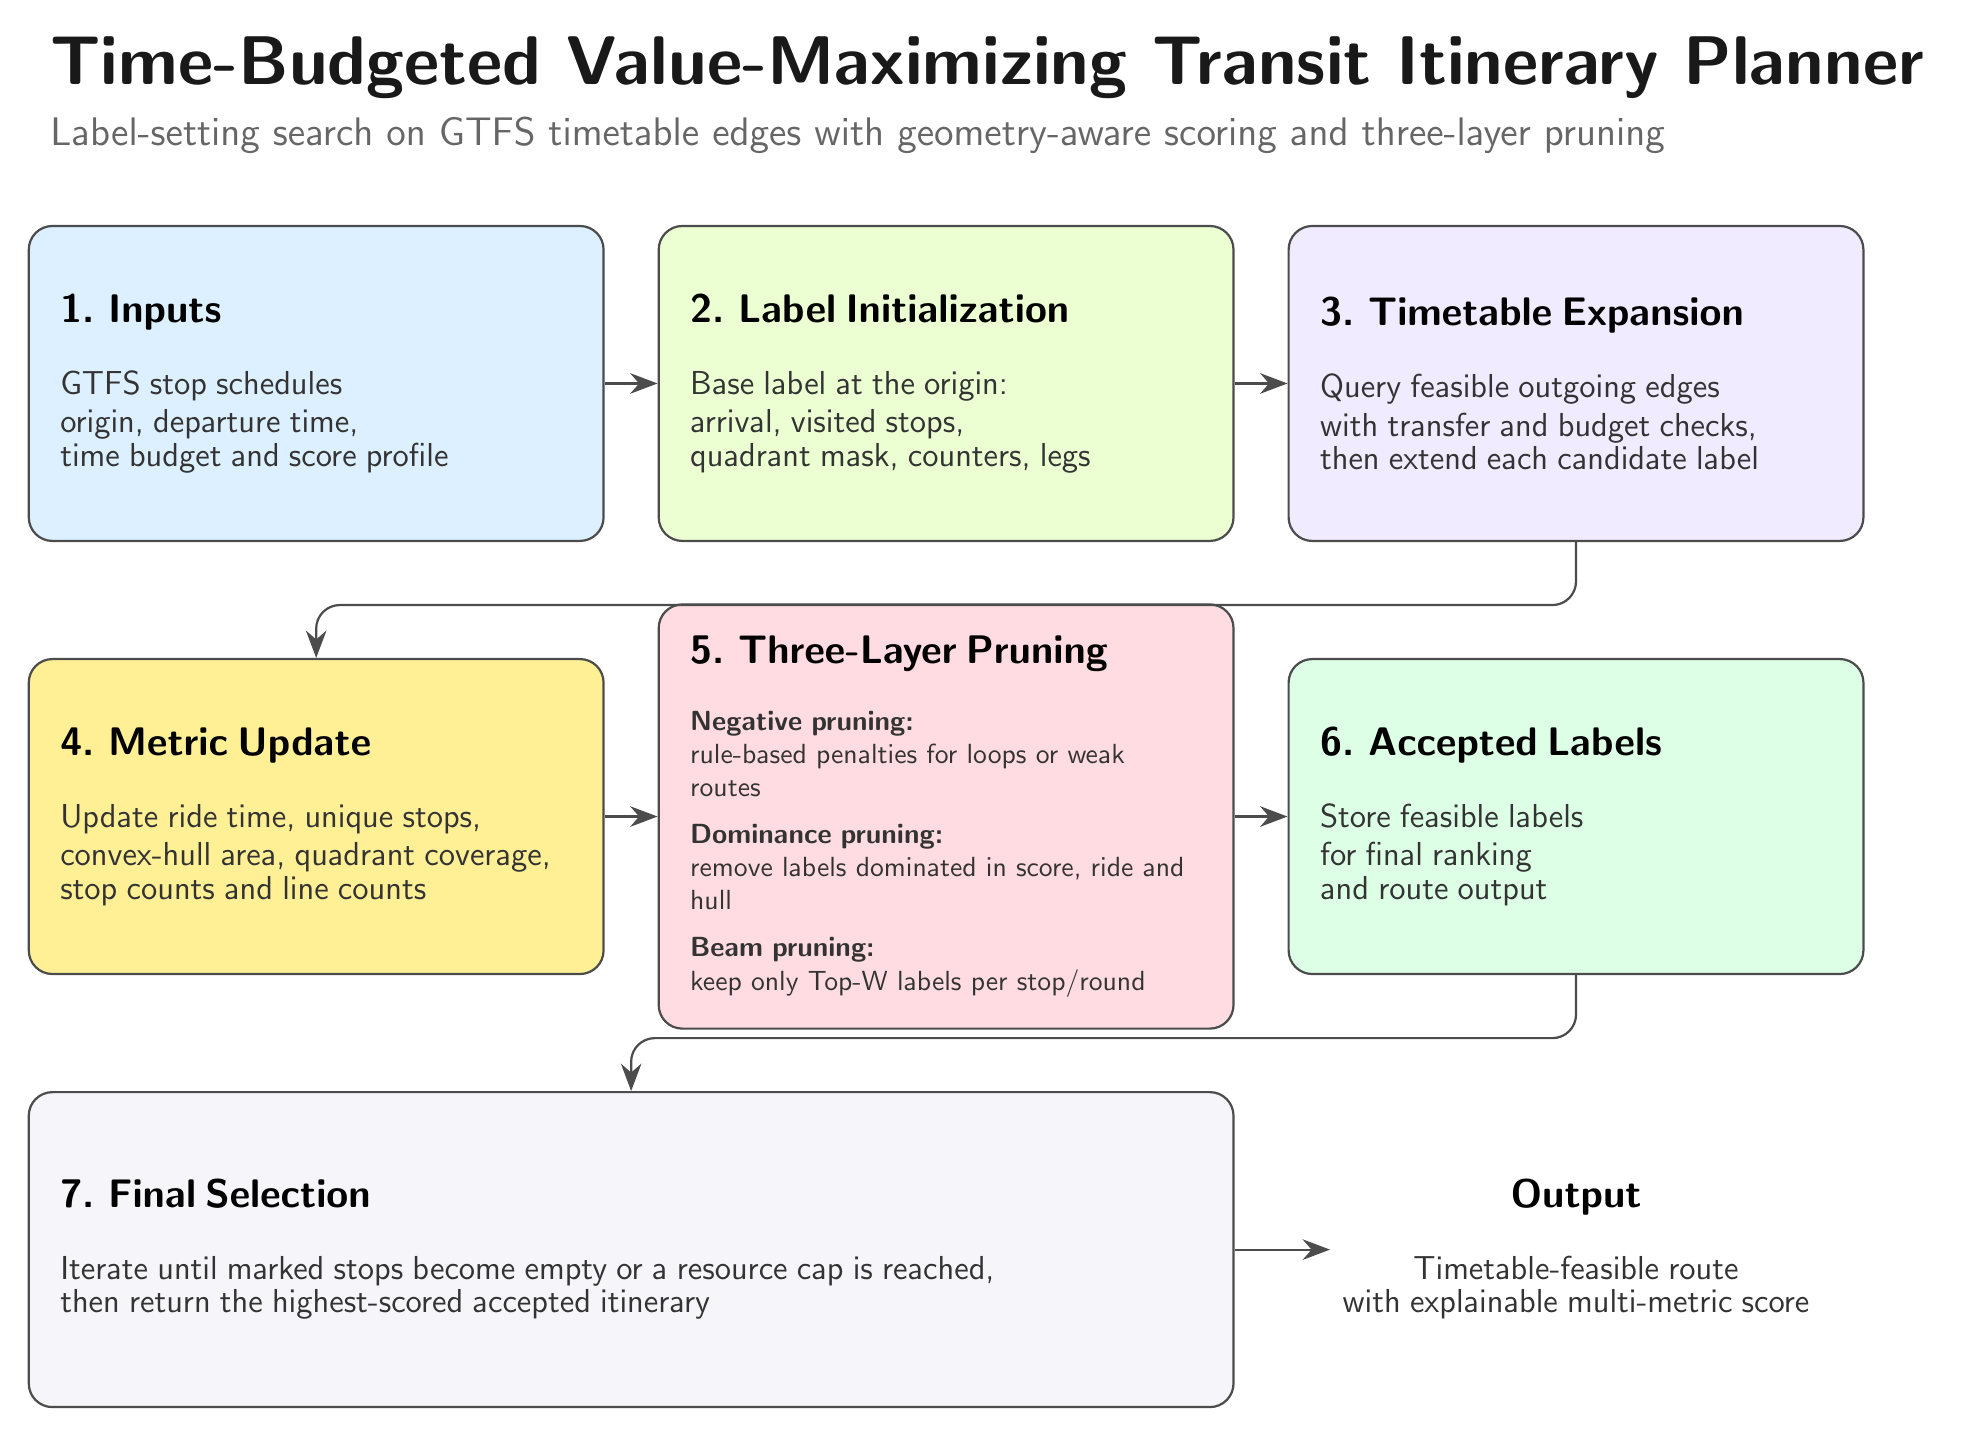
\begin{tikzpicture}[
    box/.style={draw=black!70, thick, rounded corners=3mm, fill=#1, text width=6.5cm, minimum height=4cm, align=left, inner sep=4mm},
    arrow/.style={-{Stealth[scale=1.5]}, thick, draw=black!70},
    font=\sffamily
]

% Title
\node[anchor=south west, font=\Huge\bfseries, text=black!90] (title) at (-3.5, 3.5) {Time-Budgeted Value-Maximizing Transit Itinerary Planner};
\node[anchor=north west, font=\Large, text=black!60] (subtitle) at (title.south west) {Label-setting search on GTFS timetable edges with geometry-aware scoring and three-layer pruning};

% Row 1
\node[box=b1] (box1) at (0, 0) {
    \textbf{\Large 1. Inputs}\\[12pt]
    \large\textcolor{black!80}{GTFS stop schedules\\origin, departure time,\\time budget and score profile}
};

\node[box=b2] (box2) at (8, 0) {
    \textbf{\Large 2. Label Initialization}\\[12pt]
    \large\textcolor{black!80}{Base label at the origin:\\arrival, visited stops,\\quadrant mask, counters, legs}
};

\node[box=b3] (box3) at (16, 0) {
    \textbf{\Large 3. Timetable Expansion}\\[12pt]
    \large\textcolor{black!80}{Query feasible outgoing edges\\with transfer and budget checks,\\then extend each candidate label}
};

% Row 2
\node[box=b4] (box4) at (0, -5.5) {
    \textbf{\Large 4. Metric Update}\\[12pt]
    \large\textcolor{black!80}{Update ride time, unique stops,\\convex-hull area, quadrant coverage,\\stop counts and line counts}
};

\node[box=b5] (box5) at (8, -5.5) {
    \textbf{\Large 5. Three-Layer Pruning}\\[12pt]
    \normalsize\textcolor{black!80}{\textbf{Negative pruning:}\\rule-based penalties for loops or weak routes\\[5pt]\textbf{Dominance pruning:}\\remove labels dominated in score, ride and hull\\[5pt]\textbf{Beam pruning:}\\keep only Top-W labels per stop/round}
};

\node[box=b6] (box6) at (16, -5.5) {
    \textbf{\Large 6. Accepted Labels}\\[12pt]
    \large\textcolor{black!80}{Store feasible labels\\for final ranking\\and route output}
};

% Row 3
\node[box=b7, text width=14.5cm] (box7) at (4, -11) {
    \textbf{\Large 7. Final Selection}\\[12pt]
    \large\textcolor{black!80}{Iterate until marked stops become empty or a resource cap is reached,\\then return the highest-scored accepted itinerary}
};

\node[text width=6cm, align=center] (box8) at (16, -11) {
    \textbf{\Large Output}\\[12pt]
    \large\textcolor{black!80}{Timetable-feasible route\\with explainable multi-metric score}
};

% Connections
\draw[arrow] (box1) -- (box2);
\draw[arrow] (box2) -- (box3);

\draw[arrow, rounded corners=3mm] (box3.south) -- +(0,-0.8) -| (box4.north);

\draw[arrow] (box4) -- (box5);
\draw[arrow] (box5) -- (box6);

\draw[arrow, rounded corners=3mm] (box6.south) -- +(0,-0.8) -| (box7.north);

\draw[arrow] (box7) -- (box8);

\end{tikzpicture}
\end{document}
